\documentclass[12pt, spanish]{article}
\usepackage[spanish]{babel}
\selectlanguage{spanish}
%\usepackage{natbib}
\usepackage{url}
\usepackage[utf8x]{inputenc}
\usepackage{graphicx}
\graphicspath{{images/}}
\usepackage{parskip}
\usepackage{fancyhdr}
\usepackage{vmargin}
\usepackage{multirow}
\usepackage{float}
\usepackage{chngpage}

\usepackage{amsfonts}

\usepackage{subcaption}

\usepackage{hyperref}
\usepackage[
    type={CC},
    modifier={by-nc-sa},
    version={4.0},
]{doclicense}

\hypersetup{
    colorlinks=true,
    linkcolor=blue,
    filecolor=magenta,      
    urlcolor=cyan,
}

% para codigo
\usepackage{listings}
\usepackage{xcolor}



%% configuración de listings

\definecolor{listing-background}{HTML}{F7F7F7}
\definecolor{listing-rule}{HTML}{B3B2B3}
\definecolor{listing-numbers}{HTML}{B3B2B3}
\definecolor{listing-text-color}{HTML}{000000}
\definecolor{listing-keyword}{HTML}{435489}
\definecolor{listing-identifier}{HTML}{435489}
\definecolor{listing-string}{HTML}{00999A}
\definecolor{listing-comment}{HTML}{8E8E8E}
\definecolor{listing-javadoc-comment}{HTML}{006CA9}

\lstdefinestyle{eisvogel_listing_style}{
  language         = python,
%$if(listings-disable-line-numbers)$
%  xleftmargin      = 0.6em,
%  framexleftmargin = 0.4em,
%$else$
  numbers          = left,
  xleftmargin      = 0em,
 framexleftmargin = 0em,
%$endif$
  backgroundcolor  = \color{listing-background},
  basicstyle       = \color{listing-text-color}\small\ttfamily{}\linespread{1.15}, % print whole listing small
  breaklines       = true,
  frame            = single,
  framesep         = 0.19em,
  rulecolor        = \color{listing-rule},
  frameround       = ffff,
  tabsize          = 4,
  numberstyle      = \color{listing-numbers},
  aboveskip        = 1.0em,
  belowskip        = 0.1em,
  abovecaptionskip = 0em,
  belowcaptionskip = 1.0em,
  keywordstyle     = \color{listing-keyword}\bfseries,
  classoffset      = 0,
  sensitive        = true,
  identifierstyle  = \color{listing-identifier},
  commentstyle     = \color{listing-comment},
  morecomment      = [s][\color{listing-javadoc-comment}]{/**}{*/},
  stringstyle      = \color{listing-string},
  showstringspaces = false,
  escapeinside     = {/*@}{@*/}, % Allow LaTeX inside these special comments
  literate         =
  {á}{{\'a}}1 {é}{{\'e}}1 {í}{{\'i}}1 {ó}{{\'o}}1 {ú}{{\'u}}1
  {Á}{{\'A}}1 {É}{{\'E}}1 {Í}{{\'I}}1 {Ó}{{\'O}}1 {Ú}{{\'U}}1
  {à}{{\`a}}1 {è}{{\'e}}1 {ì}{{\`i}}1 {ò}{{\`o}}1 {ù}{{\`u}}1
  {À}{{\`A}}1 {È}{{\'E}}1 {Ì}{{\`I}}1 {Ò}{{\`O}}1 {Ù}{{\`U}}1
  {ä}{{\"a}}1 {ë}{{\"e}}1 {ï}{{\"i}}1 {ö}{{\"o}}1 {ü}{{\"u}}1
  {Ä}{{\"A}}1 {Ë}{{\"E}}1 {Ï}{{\"I}}1 {Ö}{{\"O}}1 {Ü}{{\"U}}1
  {â}{{\^a}}1 {ê}{{\^e}}1 {î}{{\^i}}1 {ô}{{\^o}}1 {û}{{\^u}}1
  {Â}{{\^A}}1 {Ê}{{\^E}}1 {Î}{{\^I}}1 {Ô}{{\^O}}1 {Û}{{\^U}}1
  {œ}{{\oe}}1 {Œ}{{\OE}}1 {æ}{{\ae}}1 {Æ}{{\AE}}1 {ß}{{\ss}}1
  {ç}{{\c c}}1 {Ç}{{\c C}}1 {ø}{{\o}}1 {å}{{\r a}}1 {Å}{{\r A}}1
  {€}{{\EUR}}1 {£}{{\pounds}}1 {«}{{\guillemotleft}}1
  {»}{{\guillemotright}}1 {ñ}{{\~n}}1 {Ñ}{{\~N}}1 {¿}{{?`}}1
  {…}{{\ldots}}1 {≥}{{>=}}1 {≤}{{<=}}1 {„}{{\glqq}}1 {“}{{\grqq}}1
  {”}{{''}}1
}
\lstset{style=eisvogel_listing_style}


\usepackage[default]{sourcesanspro}

\setmarginsrb{2 cm}{1 cm}{2 cm}{2 cm}{1 cm}{1.5 cm}{1 cm}{1.5 cm}

\title{Práctica 3:\\
Programación  \hspace{0.05cm} }                           
\author{Antonio David Villegas Yeguas}                             
\date{\today}                                           

\renewcommand*\contentsname{hola}

\makeatletter
\let\thetitle\@title
\let\theauthor\@author
\let\thedate\@date
\makeatother

\pagestyle{fancy}
\fancyhf{}
\rhead{\theauthor}
\lhead{\thetitle}
\cfoot{\thepage}

\begin{document}

%%%%%%%%%%%%%%%%%%%%%%%%%%%%%%%%%%%%%%%%%%%%%%%%%%%%%%%%%%%%%%%%%%%%%%%%%%%%%%%%%%%%%%%%%

\begin{titlepage}
    \centering
    \vspace*{0.3 cm}
    
\includegraphics[scale = 0.50]{ugr.png}\\[0.7 cm]
    %\textsc{\LARGE Universidad de Granada}\\[2.0 cm]   
    \textsc{\large 3º CSI 2019/20 - Grupo 1}\\[0.5 cm]            
    \textsc{\large Grado en Ingeniería Informática}\\[0.5 cm]              
    \rule{\linewidth}{0.2 mm} \\[0.2 cm]
    { \huge \bfseries \thetitle}\\
    \rule{\linewidth}{0.2 mm} \\[1 cm]
    
    \begin{minipage}{0.4\textwidth}
        \begin{flushleft} \large
            \emph{Autor:}\\
            \theauthor\\ 
			 \emph{DNI:}\\
            77021623-M
            \end{flushleft}
            \end{minipage}~
            \begin{minipage}{0.4\textwidth}
            \begin{flushright} \large
            \emph{Asignatura: \\
            AA}   \\     
            \emph{Correo:}\\
            advy99@correo.ugr.es           
        \end{flushright}
    \end{minipage}\\[0.5cm]
  
    {\large \thedate}\\[0.5cm]
    %{\url{https://github.com/advy99/AA/}}
    {\doclicenseThis}
 	
    \vfill
    
\end{titlepage}

%%%%%%%%%%%%%%%%%%%%%%%%%%%%%%%%%%%%%%%%%%%%%%%%%%%%%%%%%%%%%%%%%%%%%%%%%%%%%%%%%%%%%%%%%

\tableofcontents
\pagebreak

%%%%%%%%%%%%%%%%%%%%%%%%%%%%%%%%%%%%%%%%%%%%%%%%%%%%%%%%%%%%%%%%%%%%%%%%%%%%%%%%%%%%%%%%%


\section*{Introducción}

Para esta práctica se pide explicar el proceso a realizar para resolver dos problemas de aprendizaje utilizando los modelos lineales vistos a lo largo de la teoría y prácticas de la asignatura.

Para esta práctica utilizaré la biblioteca Scikit-Learn\cite{sklearn} ya que cuenta con todas las herramientas que utilizaré y explicaré más adelante. No usé esta herramienta en prácticas anteriores ya que se nos pedía implementar los algoritmos y herramientas, sin embargo para esta práctica nos será más sencillo utilizarla.

\begin{quote}
\textit{``Que trabajen los romanos que para eso tienen el pecho de lata.''} -  Anónimo.
\end{quote}

\section{Problema de clasificación.}

\subsection{Comprender el problema. Identificar X, Y y F en el problema.}

En este problema tenemos datos sobre imágenes de números escritos a mano por un total de 43 personas, los números escritos por 30 de estas son el conjunto de training dado y los números de las 13 personas restantes conforman el conjunto de test. Estos datos se han obtenido de la base de datos \textit{Machine Learning Repository}, en concreto usaremos el conjunto de datos \textit{Optical Recognition of Handwritter Digits Data Set} \cite{mlr_digitos}.

Cada número se representa como una imagen de 32 por 32 bitmaps, donde 1 representa que en dicha posición se ha escrito y un 0 no. Como podemos leer en la descripción del \textit{data set}, los datos que usamos están preprocesados, en lugar de tener una matriz 32 por 32 se han separado en bloques de 4 por 4 sin solapamiento de forma que tenemos una matriz 8 por 8, 64 valores entre 0 a 16,0 si el bloque no tiene ningún pixel en negro y 16 si todos los píxeles del bloque son negros.

Los ficheros de datos de entrada cuentan con 65 columnas por cada fila, los 64 valores de la imagen y por último la clase a la que pertenece dicho dato. Explicaré que significa cada valor y que clases posibles pueden tomar en las siguientes secciones.

Con respecto al problema, debemos ser conscientes de que con gran seguridad contarán con ruido ya que la forma de escritura de cada persona será distinto, y habrá imágenes muy parecidas que sin embargo sean de clase distintas.

\subsubsection{X del problema.}

El conjunto X del problema son los datos de entrada con los que entrenaremos el modelo. 

Como leemos del fichero de información de descripción disponible en la base de datos\cite{mlr_digitos}, cada dato x cuenta con 64 variables cuyo valor está en el rango [0,16], cada variable representa una sección 4 por 4 de la imagen leída del número, si el valor es 16 quiere decir que la sección está por completo escrita, y un 0 que ninguno de sus píxeles está escrito el valor.

Comprobaremos que esto efectivamente es así cuando hablemos sobre los conjuntos de training y test más adelante.

\subsubsection{Y del problema.}

Las etiquetas del problema representan los valores escritos en la entrada, es decir, un dato leído tendrá sus 64 valores correspondientes a la información de la imagen leída y la etiqueta será un valor entre [0,9] que representa el valor escrito en la imagen.

\subsubsection{F del problema.}

La función $f$ del problema es la función desconocida que clasifica de forma perfecta cualquier número. El objetivo de esta práctica es obtener una función $g$ perteneciente al conjunto de clases de funciones a usar (del que hablaré más adelante) que sea lo más parecida posible a la función $f$.

Este problema lo podemos tratar como un problema de aprendizaje ya que los datos cuentan con un patrón (si a una entrada le damos una etiqueta es muy probable que las entradas similares tengan la misma etiqueta), la función $f$ es desconocida y no es calculable, ya que si lo fuera no necesitamos utilizar técnicas de aprendizaje, simplemente aplicamos la función y hemos resuelto el problema, y por último, tenemos datos con los que entrenar nuestro modelo.

\subsection{Clases de funciones a usar.}

Para este problema utilizaré combinaciones lineales de los datos. Dado que las características de los datos de entrada son la cantidad de unos que hay en una zona de la matriz que representa la imagen no tiene sentido aplicar transformaciones no lineales a los valores, es decir, no tiene ningún significado aplicar el cuadrado a un número de bits.

Otra razón es que el problema ya es de gran dimensionalidad, si usamos clases de funciones más complejas podría presentar problemas de overfitting o una necesidad mayor de tiempo de entrenamiento.

\subsection{Conjuntos de training y test.}

El problema ya nos proporciona un conjunto de training y test separado, luego no tendremos que separarlos para este problema.

Para leer los ficheros, al tener el formato de fichero CSV (aunque la extensión no sea CSV), he utilizado la biblioteca pandas, en concreto el método \texttt{read\_csv}\cite{pandasReadCSV}.

Al leer los ficheros, el conjunto de datos X serán las distintas filas con todas las columnas a excepción de la última y el conjunto de etiquetas serán la última columna de todas las filas.

\subsubsection{Conjunto de training}

Tras leer los ficheros dados de training podemos comprobar los datos del problema. En este caso el conjunto dado de training cuenta con 3823 datos y como vimos en la introducción del problema, podemos comprobar que efectivamente cada dato tiene 64 variables:

\begin{figure}[H]
	\centering
	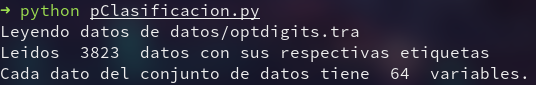
\includegraphics[scale=0.7]{clasificacion/num_datos.png}
	\caption{Información sobre el número de datos en training.}
	\label{datosClasificacion}
\end{figure}

De la lectura de este fichero también podemos ver el reparto de los datos según su clase al estar realizando técnicas de aprendizaje supervisado (como hemos hecho en anteriores prácticas y también haremos en esta):

\begin{figure}[H]
	\centering
	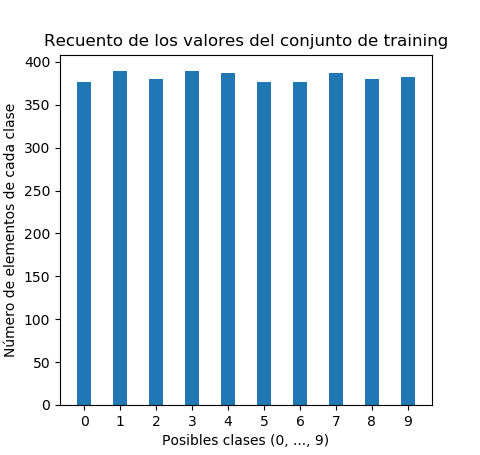
\includegraphics[scale=1]{clasificacion/datos_tra.png}
	\caption{Información sobre la clase de los datos en training.}
	\label{claseDatosClasificacion}
\end{figure}

Como podemos ver el número de elementos de cada clase está equilibrado, luego en principio no debería generar problemas al entrenar nuestro modelo. Es importante que en el conjunto de training se de este equilibrio y se encuentren datos de todas las clases, ya que en caso contrario podría ocurrir que en el conjunto de test o incluso fuera de la muestra fallemos al intentar clasificar un dato que contiene información sobre una clase desconocida al entrenar, pero como podemos ver, este no es el caso.

\subsubsection{Conjunto de validación}

A partir del conjunto de entrenamiento obtendré un conjunto para realizar la validación del modelo. Usaré cross-validation a través de las herramientas que ofrece Scitik-Learn para realizar la validación cruzada\cite{crossval}, aunque comentaré en la sección de hiperparámetros el número de particiones de validación. 

Este método consiste en dividir los datos de entrenamiento, de forma que tengamos un conjunto de entrenamiento más pequeño y $k$ conjuntos de validación ($k$ es un entero que discutiré en la sección de hiperparámetros), de forma que se entrenará $k$  veces y se validará con las $k$ particiones de validación, y finalmente nos quedaremos con la media de estas, para asegurar tener un buen ajuste.

\subsubsection{Conjunto de test}

En el fichero que nos proporcionan con los datos de test vemos que tenemos 1797 datos (bastantes menos que en el conjunto de training), pero como es de esperar, cada dato usa la misma representación, es decir, está compuesto por 64 características y la clase a la que pertenece:

\begin{figure}[H]
	\centering
	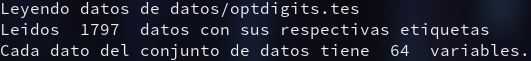
\includegraphics[scale=0.7]{clasificacion/num_datos_test.png}
	\caption{Información sobre el número de datos  en test.}
	\label{datosClasificacionTest}
\end{figure}


Con respecto al número de datos por clase, en este conjunto también vemos que tenemos una distribución uniforme de los datos entre las clases, aunque en este caso no es importante al no usar este conjunto para el entrenamiento, es decir, este conjunto de datos solo lo usaremos para comprobar como se comportan los distintos modelos.

\begin{figure}[H]
	\centering
	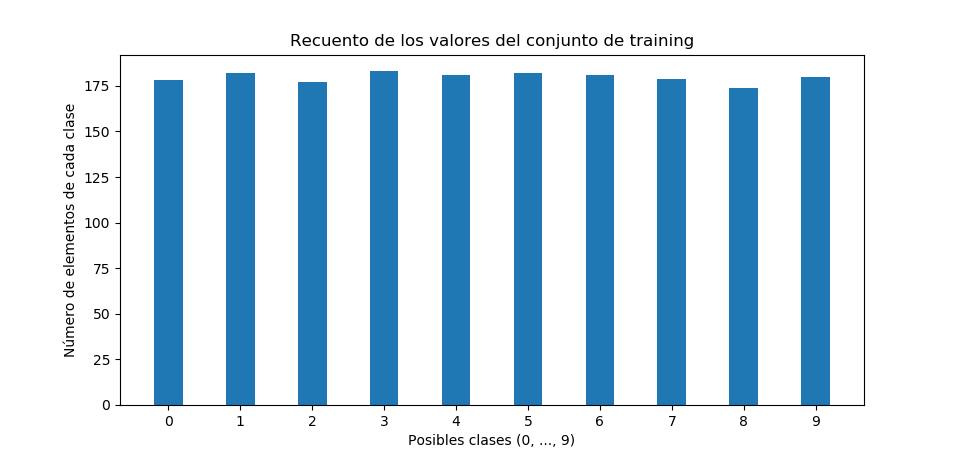
\includegraphics[scale=0.7]{clasificacion/datos_test.png}
	\caption{Información sobre la clase de los datos en test.}
	\label{claseDatosTestClasificacion}
\end{figure}

\newpage

\subsection{Preprocesado de los datos.}

Como he comentado con respecto a los datos de este problema, en el repositorio de donde se han extraído los datos nos avisan de que estos ya se encuentran preprocesados, inicialmente los datos eran un bitmap con valores 0 o 1 representado en una matriz de 32 por 32, que se ha preprocesado de forma que se ha dividido en secciones de bitmap 4 por 4 sin solapamiento, es decir, los datos ya preprocesados son una matriz con valores entre 0 y 16 en la que cada posición representa un cuadrante 4 por 4, de ahí que el valor esté entre 0 (el bitmap de la sección no tenia ningún valor como 1) a 16 (todos los valores del bitmap en esa sección 4 por 4 valen 1).

Los valores todos están en un rango fijo que es el mismo para todos (entre 0 y 16), por lo que en principio no va a afectar, por lo que no lo modificaré. Es posible que en esta sección aparezca una nota en la que si finalmente se ha obtenido mejor resultado normalizando los valores entre 0 y 1 se ha aplicado esa transformación a los datos (básicamente consiste en dividir todos los datos por 16 para que se encuentren en el rango [0, 1]).

Además de este motivo, no voy a realizar preprocesado de datos ya que en la información del dataset se nos informa de que con ese preprocesado los datos se comportan de manera correcta, es decir, que en principio no debería haber problemas, aun así si observo que no logramos unos resultados adecuados ampliaré esta sección para intentar aplicar un preprocesado que nos mejore los resultados.

Tras realizar pruebas he decidido mantenerme en la misma posición ya que con esta se obtienen resultados muy buenos, y aplicando algún tipo de preprocesado como por ejemplo normalización entre 0 y 1 de los valores se empeora los resultados.

\subsection{Fijar la métrica. Idoneidad sobre el problema.}

En este apartado fijaremos la métrica que usaremos para la evaluación, es decir, la métrica que utilizaremos para calcular el error del modelo una vez esté entrenado, es decir, saber como bien se comporta. Esto no quiere decir que la métrica que usará el modelo para entrenarse sea esta, ya que como veremos usaremos una distinta, lo cual justificaré más adelante.

Debido a que estamos en un problema de clasificación la métrica de evaluación será la tasa de aciertos, es decir, la tasa de datos que asigna la etiqueta correcta. He hecho esta elección ya que no nos interesa saber un valor numérico sobre cuanto se ha equivocado, si no si es capaz de clasificar los puntos bien.



\subsection{Técnica de ajuste elegida.}

Para realizar el ajuste usaremos la métrica Mean Squared Error, ya que los modelos lineales que he seleccionado y veremos más adelante se basan en regresión (aunque algunos sean variaciones para clasificación, en realidad usan regresión), luego no podemos usar la métrica para la evaluación escogida. 

Usaremos esta métrica de ajuste ya que es bastante conocida para nosotros y la hemos utilizado en otras prácticas de clasificación en las que hemos usado modelos lineales basados en regresión, además de ser el error usado en la prueba de la que nos habla la descripción del dataset.


$$ \frac{1}{N} \sum_{i=1}^{N}{(y_i - \hat{y}_i)^2} $$

Siendo $y_i$ la clase real del dato e $\hat{y}_i$ la clase predecida por el modelo.

Tras realizar diversos experimentos que comentaré más adelante en la selección de hiperparámetros, usando la métrica de mínimos cuadrados en gradiente descendente estocástico obtenemos muy malos resultados, por este motivo usaré también la métrica Hinge\cite{hingeLoss} para este modelo.

Esta métrica consiste en obtener un Support Vector Machine lineal, que nos definirá la función de perdida y el vector de pesos se verá modificado acorde a dicho SVM.

\subsection{Necesidad de regularización.}

La regularización es necesaria para evitar el overfitting al entrenar el modelo. La idea de utilizar regularización es minimizar el cambio en la función de error, para obligar a que no se ajuste de forma perfecta a los datos. Esta técnica nos será útil especialmente cuando los datos contienen ruido, como es nuestro caso.

Debido a la alta dimensionalidad de los datos, a pesar de no utilizar un conjunto de clases de funciones complejos, es posible que se genere overfitting, aunque no lo sabemos a priori, por este motivo en los modelos a usar que explicaré más adelante probaré a utilizar los distintos modelos con y sin regularización.

En principio si es necesaria esta regularización, sin embargo voy a realizar distintos experimentos para comprobar su importancia.

Para aplicar la regularización existen dos normas\cite{l1l2regularizacion}.


\subsubsection{Norma L1: }

La norma L1, llamada Regresión Lasso, consiste en añadir el valor absoluto de la magnitud multiplicado por el coeficiente de penalización:

$$ \lambda \sum_{j=1}^{p}{|\beta_j|} $$

\subsubsection{Norma L2:}

La norma L2, también llamada Ridge Regression, se basa en añadir el cuadrado de la magnitud por el coeficiente de penalización en la función de coste:

$$ \lambda \sum_{j=1}^{p}{\beta_j^2} $$


En este problema utilizaremos la norma L2 ya que es la más similar a la métrica de ajuste usada. En caso de que al realizar pruebas y comprobar que la norma L1 se comporta mejor, modificaré esta sección explicando el cambio (si se llega a producir).

\newpage

\subsection{Modelos a usar.}

En esta sección comentaré los modelos lineales a usar para intentar resolver el problema.

Usaré Regresión Lineal con regularización (Ridge Regression), Regresión Logística y Gradiente Descendente Estocástico. Usaré la implementación dada en Scikit-Learn\cite{scikitlearnlinearmodels}, y comentaré como funcionan, aunque son los algoritmos vistos en prácticas anteriores por los que ya los conocemos.

He decidido no usar el modelo Perceptron ya que, como he comentado, los datos pueden contener ruido y no ser linealmente separables, aun así podría haber usado el modelo PLA-Pocket, sin embargo considero que estudiando el comportamiento en los cuatro modelos mencionados no es necesario añadir este, así como tampoco usar Regresión Lineal, ya que la he sustituido por la versión con regularización al poder adaptar la regularización a través de sus hiperparámetros, y en caso de no querer regularizar simplemente el parámetro del peso de la regularización será 0.


\subsubsection{Clasificación Ridge.}

Este modelo es una variación de la Regresión Lineal pero teniendo en cuenta la regularización. En concreto usa la norma L2. Como podemos ver en su código fuente\cite{sourceRidge}, se trata del modelo anterior teniendo en cuenta dicha norma.

Aunque en principio se trata de una variación de Regresión Lineal, cuenta con una variación para clasificación que es la citada en esta memoria, y que usaremos para este problema al ser de clasificación. Esta variación simplemente convierte las etiquetas en valores 1 o -1 y aplica el método de regresión. Para problemas multiclase como es el nuestro, automáticamente  aplicará $n$ veces el algoritmo siendo $n$ el número de clases, de forma que cada ejecución el valor 1 será una clase y el valor -1 las clases restantes.


\subsubsection{Regresión Logística.}

En este caso este modelo es el visto en otras prácticas y en teoría, pero con la diferencia de que al usar los recursos de Scikit-Learn\cite{sourceLogistic} tienen en cuenta un mayor número de hiperparámetros que nosotros no tuvimos en cuenta, los cuales discutiré más adelante.

\subsubsection{Gradiente Descendente Estocástico.}

De nuevo, este modelo es el visto en la asignatura, sin embargo Scikit-Learn cuenta con dos variantes, una para clasificación y otra para regresión. En este problema, al tratarse de clasificación, usaremos la variante de clasificación\cite{sourceSGDClas}.


\newpage

\subsection{Hiperparámetros y selección del mejor modelo.}

En esta sección discutiré los hiperparámetros de cada algoritmo, así como cuales considero los mejores para cada uno, y finalmente el modelo que mejor se comportan en nuestro problema.

Para realizar las ejecuciones, como he comentado, usaré Scikit-Learn. Para realizar una ejecución tiene distintos pasos:

\begin{enumerate}
	\item Declaración del modelo a utilizar. Debemos crear una variable que tendrá un objeto de la clase del modelo a utilizar, en la creación de este objeto será cuando especificaremos los hiperparámetros del modelo.
	\item Ajustar el modelo haciendo uso del método fit de la clase de dicho modelo. Se encargará de estimar el modelo.
	\item Calcular el error dentro de la muestra usando validación cruzada. Esto lo haremos haciendo uso del método \texttt{cross\_val\_score}.
	\item Predecir las etiquetas del conjunto de test.
	\item Calcular el error en el conjunto de test.
\end{enumerate}

Un ejemplo sería:

\begin{lstlisting}
estimador = ClaseEstimador(hiperparametros)
print("\tAjustando el modelo")
estimador.fit(x,y)
# aplicamos validación cruzada una vez tenemos el modelo ajustado
print("\tAplicando", cv, "-k-folds cross-validation")
# usamos de metrica la tasa de aciertos (accuracy)
resultado_cross_val = cross_val_score(estimador, x, y, scoring='accuracy', cv=cv)
fin = time.time()
print("\tTiempo (en segundos) necesario para ajustar el modelo y aplicar cross-validation: ", fin-inicio)
print("\n")
print("\tEvaluación media de aciertos usando cross-validation: ", resultado_cross_val.mean())
print("\tE_in usando cross-validation: ", 1-resultado_cross_val.mean())

print("\tPrediciendo las etiquetas en test")
# predecimos test acorde al modelo
y_predecida_test = clasificador.predict(x_test).round()
# miramos la tasa de aciertos, es decir, cuantos ha clasificado bien
print("\tObteniendo E_test a partir de la predicción")
aciertos = accuracy_score(y_test, y_predecida_test)
print("\tPorcentaje de aciertos en test: ", aciertos)
print("\tE_test: ", 1-aciertos)
\end{lstlisting}

Ya que la única diferencia entre usar un modelo u otro es la primera linea, y además fijamos los hiperparámetros, lo he separado en una función donde le pasamos el estimador:

\begin{lstlisting}
estimador = ClaseEstimador(hiperparametros)
evaluar(estimador, x, y, x_test, x_test, num_kfolds)
\end{lstlisting}

\subsubsection{Clasificación Ridge.}

En este modelo, aunque ofrece gran cantidad de parámetros para controlar su funcionamiento, nos vamos a centrar en tres:

\begin{enumerate}
	\item alpha: Factor por el que se multiplica el método de regularización, en este caso la norma L2 aplicada por defecto. Este parámetro por defecto tiene valor 1.
	\item max\_iter: Máximo número de iteraciones del algoritmo. Por defecto no tiene límite de iteraciones.
	\item tol: Precisión de la solución. Por defecto $1^{-3}$.
\end{enumerate}


Podemos ver todos los parámetros disponibles en la web de Scikit-Learn\cite{ridge}.


Para este modelo no modificaré la precisión de la solución ya que es bastante baja ni el máximo de iteraciones ya que no consume un tiempo considerable.

El factor que si modificaré será el factor que multiplica al método de regularización. He realizado pruebas con valores 0 (sin regularización), 0.1, 1 (valor por defecto) y 2, obteniendo estos resultados:



\begin{figure}[H]
	\centering
	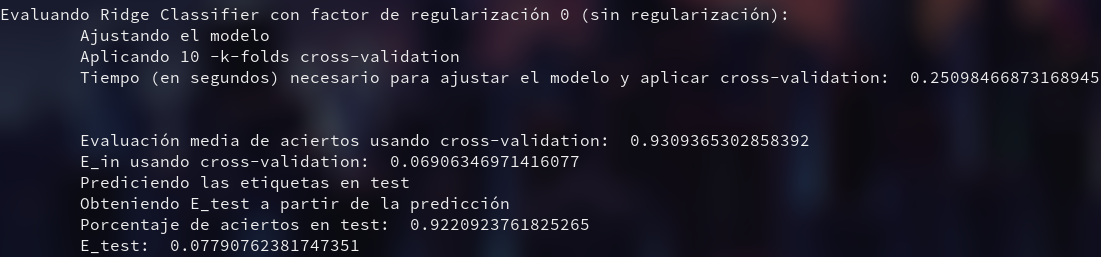
\includegraphics[scale=0.45]{clasificacion/ridge0.png}
	\caption{Resultado usando el algoritmo Ridge Classifier sin regularización.}
	\label{ridge0}
\end{figure}


\begin{figure}[H]
	\centering
	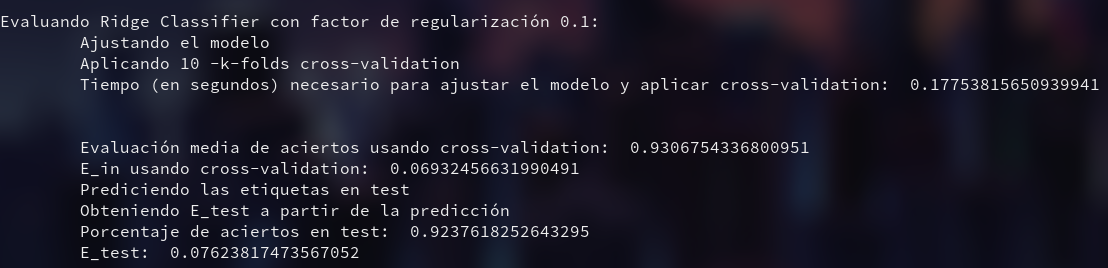
\includegraphics[scale=0.45]{clasificacion/ridge01.png}
	\caption{Resultado usando el algoritmo Ridge Classifier con factor de regularización 0.1.}
	\label{ridge01}
\end{figure}



\begin{figure}[H]
	\centering
	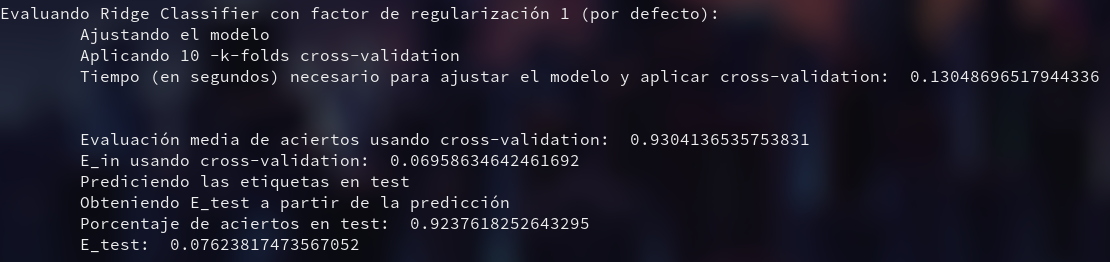
\includegraphics[scale=0.45]{clasificacion/ridge1.png}
	\caption{Resultado usando el algoritmo Ridge Classifier con factor de regularización 1.}
	\label{ridge1}
\end{figure}



\begin{figure}[H]
	\centering
	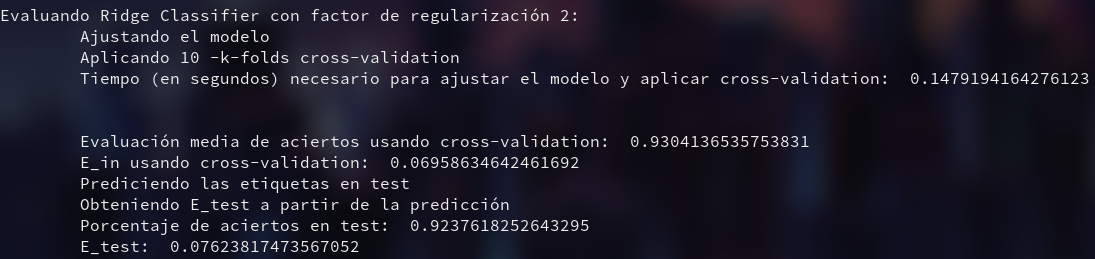
\includegraphics[scale=0.45]{clasificacion/ridge2.png}
	\caption{Resultado usando el algoritmo Ridge Classifier con factor de regularización 2.}
	\label{ridge2}
\end{figure}


En principio, viendo los resultados, vemos como este algoritmo se comporta muy bien, dando una tasa de error muy baja.

En este algoritmo podemos ver como el uso de regularización es notable, y es que en el modelo en el que no se aplicaba regularización, aunque el error dentro de la muestra es menor, el error en el conjunto de test es mayor que en los ajustes en los que se ha aplicado regularización, lo que nos da señales de overfitting, aunque es muy leve y aun sin regularización obtenemos buenos resultados.


\newpage

\subsubsection{Regresión Logística.}

Para este modelo estos serán los hiperparámetros que utilizaré:

\begin{enumerate}
	\item solver: Se trata del algoritmo a utilizar para el problema de optimización.
	\item penalty: Penalización para el ajuste, es decir, la regularización, puede tomar valores L1 o L2. 
	\item multi\_class: Indicar si el problema es multiclase.
	\item max\_iter: Máximo número de iteraciones para el algoritmo.
	\item C: Inversa del factor de regularización.
\end{enumerate}

Podemos ver todos los parámetros disponibles en la web de Scikit-Learn\cite{logisticregression}.


En principio utilizaré el solver newtown-cg ya que es el recomendado por la documentación y funciona bastante bien como veremos.

Como ya hemos comentado, para la regularización usaré la norma L2.

Nuestro problema es multiclase, luego en el atributo multi\_class tendrá el valor multinomial.

Con respecto al máximo de iteraciones, he mantenido el número por defecto (100 iteraciones) ya que no son necesarias más (en caso de que se quede sin iteraciones scikit-learn nos mostraría un aviso por pantalla, que como veremos no hace).

Por último, el parámetro con el que realizaré varios experimentos, C. Este parámetro no es como en el modelo anterior, el peso de la regularización, si no la inversa, por lo que valores cercanos a cero serán una regularización mayor, y con valores mayores será una regularización menor. Este valor no puede ser cero.

Realizaré el ajuste para valores 0.001, 1 y 2:

\begin{figure}[H]
	\centering
	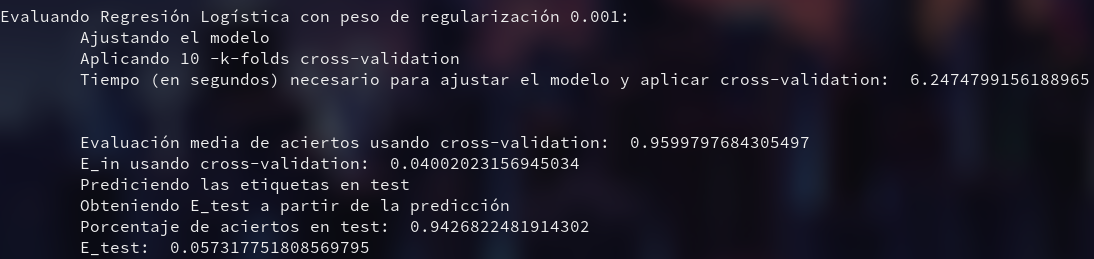
\includegraphics[scale=0.45]{clasificacion/logistic0001.png}
	\caption{Resultado usando el algoritmo Regresión Logística con factor de regularización 0.001.}
	\label{LR001}
\end{figure}


\begin{figure}[H]
	\centering
	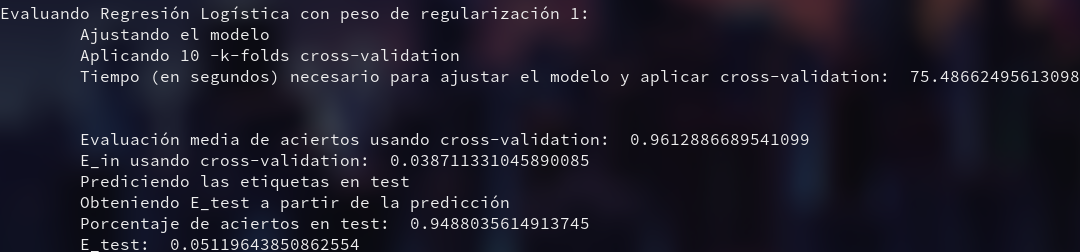
\includegraphics[scale=0.45]{clasificacion/logistic1.png}
	\caption{Resultado usando el algoritmo Regresión Logística con factor de regularización 1.}
	\label{LR1}
\end{figure}

\begin{figure}[H]
	\centering
	\hspace*{-1cm}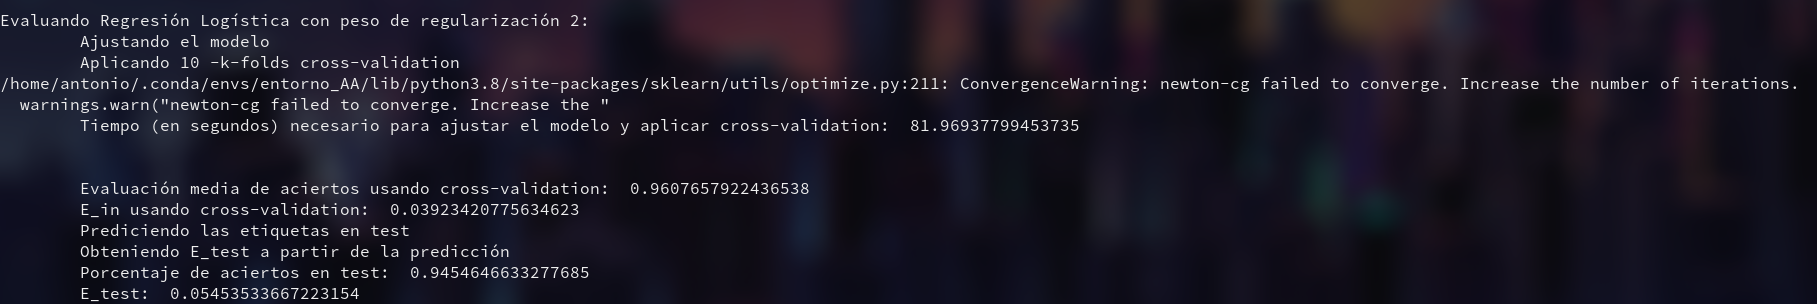
\includegraphics[scale=0.3]{clasificacion/logistic2.png}
	\caption{Resultado usando el algoritmo Regresión Logística con factor de regularización 2.}
	\label{LR2}
\end{figure}

Vemos como en este caso nos encontramos con un error en el conjunto de test menor para $C=1$, esto se debe a que con $C=0.001$ el peso de la regularización es demasiado alto, mientras que con $C=2$ es demasiado bajo, teniendo problemas de infraajuste en el primer caso y de overffiting en el segundo. Aun así, estos no son problemas grandes ni de gran importancia ya que como vemos aun así el ajuste es muy bueno.

Comentar también que en el caso de $C=2$ vemos como recibimos el aviso de que una de las 10 iteraciones de validación cruzada se ha quedado sin iteraciones, esto se debe a que en realidad está usando un número de iteraciones muy cercano al límite ya que vemos que en este problema los tiempos son mucho más altos.

\newpage

\subsubsection{Gradiente Descendente Estocástico.}

En Gradiente Descendente Estocástico tenemos los siguientes parámetros cruciales:

\begin{enumerate}
	\item loss: Función de perdida. Por defecto 'hinge'.
	\item penalty: Termino de regularización. Por defecto la norma L2.
	\item alpha: Constante multiplicadora de la regularización. Por defecto 0.0001. Con un mayor valor, mayor será la regularización.
	\item learning\_rate: Esquema para la tasa aprendizaje. Por defecto optimo, siguiendo la siguiente formula $eta = \frac{1}{alpha \cdot (t + t_0)}$ donde $t_0$ es una heurística propuesta por Leon Bottou. Como podemos ver, si el esquema es el esquema óptimo el parámetro alpha debe ser distinto a 0.
	\item eta0: Valor de la tasa de aprendizaje en caso de utilizar un esquema constante. No es usado en el esquema óptimo.
	\item max\_iter: Máximo de iteraciones del algoritmo.
\end{enumerate}

Podemos ver todos los parámetros disponibles en la web de Scikit-Learn\cite{sgdclasificacion}.

Para la función de perdida usaremos square\_loss, sin embargo, como comentamos y veremos ahora, esta función de perdida se comporta muy mal, luego también ejecutaremos el algoritmo con la función de perdida Hinge.

Para el termino de regularización, como hemos hecho con todos los modelos, usaremos la norma L2.

El parámetro alpha discutiremos más adelante cual será el mejor valor, y realizaré pruebas con valores 0, 0.0001, 0.01, 0.1 y 1.

Para el esquema de la tasa de aprendizaje realizaremos las pruebas con dos esquemas, el constante y el óptimo. Las pruebas con alpha con valor 0 solo las haré con el esquema constante ya que con el óptimo es necesario para calcular el valor de la tasa de aprendizaje.

Como nota añadir que haciendo el experimento con la función de perdida square\_loss obtenemos malos resultados siempre y voy a desechar ese modelo por sus malos resultados, así que la comparación entre el esquema constante y el óptimo será con la función de perdida Hinge.


\begin{figure}[H]
	\centering
	\hspace*{-1cm}\includegraphics[scale=0.4]{clasificacion/sgdLoss0001.png}
	\caption{Resultado usando el algoritmo SGD con factor de regularización 0.001 y función de perdida square loss.}
	\label{SGDL0001}
\end{figure}

\begin{figure}[H]
	\centering
	\hspace*{-1cm}\includegraphics[scale=0.4]{clasificacion/sgdLoss001.png}
	\caption{Resultado usando el algoritmo SGD con factor de regularización 0.01 y función de perdida square loss.}
	\label{SGDL001}
\end{figure}


\begin{figure}[H]
	\centering
	\hspace*{-1cm}\includegraphics[scale=0.4]{clasificacion/sgdLoss01.png}
	\caption{Resultado usando el algoritmo SGD con factor de regularización 0.1 y función de perdida square loss.}
	\label{SGDL01}
\end{figure}


\begin{figure}[H]
	\centering
	\hspace*{-1cm}\includegraphics[scale=0.4]{clasificacion/sgdLoss1.png}
	\caption{Resultado usando el algoritmo SGD con factor de regularización 1 y función de perdida square loss.}
	\label{SGDL1}
\end{figure}

\newpage

Vemos como este modelo, aun variando el factor de regularización, obtenemos ajustes muy malos. A continuación probamos con la función de perdida Hinge:

\begin{figure}[H]
	\centering
	\hspace*{-1cm}\includegraphics[scale=0.4]{clasificacion/sgdH001a0.png}
	\caption{Resultado usando el algoritmo SGD Classifier con tasa de aprendizaje constante 0.01, sin regularización y función de perdida Hinge.}
	\label{SGDL0}
\end{figure}

\begin{figure}[H]
	\centering
	\hspace*{-1cm}\includegraphics[scale=0.4]{clasificacion/sgdH00001.png}
	\caption{Resultado usando el algoritmo SGD Classifier con tasa de aprendizaje optima (variable) y factor de regularización 0.0001 y función de perdida Hinge.}
	\label{SGDL00001}
\end{figure}

\begin{figure}[H]
	\centering
	\hspace*{-1cm}\includegraphics[scale=0.4]{clasificacion/sgdH00001c.png}
	\caption{Resultado usando el algoritmo SGD Classifier con tasa de aprendizaje constante y factor de regularización 0.0001 y función de perdida Hinge.}
	\label{SGDL00001}
\end{figure}

\begin{figure}[H]
	\centering
	\hspace*{-1cm}\includegraphics[scale=0.4]{clasificacion/sgdH001.png}
	\caption{Resultado usando el algoritmo SGD Classifier con tasa de aprendizaje optima (variable) y factor de regularización 0.01 y función de perdida Hinge.}
	\label{SGDL001}
\end{figure}

\begin{figure}[H]
	\centering
	\hspace*{-1cm}\includegraphics[scale=0.4]{clasificacion/sgdH001c.png}
	\caption{Resultado usando el algoritmo SGD Classifier con tasa de aprendizaje constante y factor de regularización 0.01 y función de perdida Hinge.}
	\label{SGDL001}
\end{figure}


\begin{figure}[H]
	\centering
	\hspace*{-1cm}\includegraphics[scale=0.4]{clasificacion/sgdH01.png}
	\caption{Resultado usando el algoritmo SGD Classifier con tasa de aprendizaje optima (variable) y factor de regularización 0.1 y función de perdida Hinge.}
	\label{SGDL001}
\end{figure}

\begin{figure}[H]
	\centering
	\hspace*{-1cm}\includegraphics[scale=0.4]{clasificacion/sgdH01c.png}
	\caption{Resultado usando el algoritmo SGD Classifier con tasa de aprendizaje constante y factor de regularización 0.1 y función de perdida Hinge.}
	\label{SGDL001}
\end{figure}


\begin{figure}[H]
	\centering
	\hspace*{-1cm}\includegraphics[scale=0.4]{clasificacion/sgdH1.png}
	\caption{Resultado usando el algoritmo SGD Classifier con tasa de aprendizaje optima (variable) y factor de regularización 1 y función de perdida Hinge.}
	\label{SGDL001}
\end{figure}

\begin{figure}[H]
	\centering
	\hspace*{-1cm}\includegraphics[scale=0.4]{clasificacion/sgdH1c.png}
	\caption{Resultado usando el algoritmo SGD Classifier con tasa de aprendizaje constante y factor de regularización 1 y función de perdida Hinge.}
	\label{SGDL001}
\end{figure}


Vemos como en todos los casos con un esquema de tasa de aprendizaje óptimo obtenemos muy buenos resultados que se parecen mucho, los cuales ahora comentaremos.

Con el esquema constante, vemos como el factor de regularización si influye en gran medida, ya que como vemos, con un factor 1 existe demasiada regularización y por lo tanto no llega a ajustar de forma correcta el modelo, dando un error tanto en la muestra como en test bastante alto (del 40\% y 55\% respectivamente), mientras que sin regularizar obtenemos un 8'6\% de error en test, y con la regularización por defecto obtenemos un mejor valor, 5'2\% de error en test, aunque en el primero obtengamos mejor valor del error dentro de la muestra, por lo que podemos ver que la regularización sigue siendo necesaria y evita overfitting en el entrenamiento.


\subsubsection{Mejor modelo.}

Escogeré el mejor modelo según el modelo con mejor error en el conjunto de test ya que es el que mejor ha estimado unos datos con los que no ha entrenado. Por este motivo el modelo escogido será Regresión Logística con un factor de regularización $C=1$, por lo que la estimación del error se hará con este modelo.

Como conclusión también añadir que a pesar de ser necesaria la regularización, no se ha notado apenas su uso debido a que no hay gran overfitting al usar clases de funciones muy simples, aunque la dimensionalidad del problema sea alta. 

\newpage

\subsection{Estimación del error fuera de la muestra usando validación cruzada y comparación con el error en test.}

Como hemos visto tanto en teoría\cite{teoria} como en la bibliografía de la asignatura\cite{libro}, podemos hacer una estimación del error fuera de la muestra al usar validación cruzada.

Si tenemos $N$ conjuntos de validación, sabemos que:

$$E_{cv} = \frac{1}{N}\sum_{n=1}^{N}{E_{val}(g_n^-)}$$

Y como hemos visto acorde a las curvas de aprendizaje vistas en teoría, sabemos que:

$$E_{out}(g) \leq E_{cv}(g) $$

En realidad $E_{cv}$ es la media de todos los errores al usar la función \texttt{cross\_val\_score}, luego esta estimación se ha hecho para todas las pruebas que hemos realizado y en concreto en el modelo escogido obtenemos que:

$$  E_{out}(g) \leq 0'038$$

Vemos como claramente esto no es así, ya que en el mismo modelo el error en el conjunto de test es mayor (0'0512), y esto puede deberse a que el número de $k$-folds es demasiado alto.




\subsection{Modelo propuesto y estimación del error fuera de la muestra de este modelo.}

Podemos hacer una estimación del error fuera de la muestra usando el conjunto de test. En el modelo que hemos escogido vemos como esta estimación se de un error del 5'12\%.

Esto lo podemos comprobar mostrando la matriz de confusión.

Esta matriz hará un recuento de los datos reales y predecidos. En las filas se muestra el valor real de la clase, y el las columnas el valor predecido por nuestro modelo, de forma que si el valor real es un 0 y el modelo ha predecido un 7, sumará uno en la posición 0,7. 

\begin{figure}[H]
	\centering
	\includegraphics[scale=0.45]{clasificacion/matrizC.png}
	\caption{Matriz de confusión con los datos predecidos del modelo seleccionado.}
	\label{MC}
\end{figure}

El que en esta matriz se muestre la diagonal con los números mayores quiere decir que la mayor parte del conjunto de test ha realizado una buena predicción, mientras que en las posiciones  fuera de la diagonal ha cometido error. Vemos como principalmente comete errores al clasificar el número 8, que lo suele confundir con un 1 (imagino que al ser ambos bastante similares, ser simétricos y estar por la zona central de la imagen) y con un 9 (al compartir la misma zona de la imagen y solo diferenciarse en un cuadrante de la imagen).

Aun así, hemos obtenido muy buenos resultados para ser un problema con gran número de variables y tener gran cantidad de clases.

\newpage

\section{Problema de regresión.}
\subsection{Comprender el problema. Identificar X, Y y F en el problema.}

Para este problema tenemos datos distintas comunidades de Estados Unidos donde nos dan información sobre la población y como meta el número de crímenes violentos por población. Este conjunto cuenta con 1994 instancias y cada instancia con 128 atributos, aunque nos avisan de que algunos de estos no son predictivos. Estos datos se han obtenido de la base de datos \textit{Machine Learning Repository}, en concreto usaremos el conjunto de datos \textit{Communities and Crime Data Set} \cite{mlr_crimen}.


De entre las variables predictoras podemos encontrar la población de cada comunicadad, los ingresos según raza, coste medio de vivir en dicha zona, porcentaje de policías según la raza, porcentaje de población inmigrante, entre muchos otros factores. Discutiré los datos con más profundidad en los siguientes apartados.


Con respecto al problema, debemos ser conscientes de que con gran seguridad contarán con ruido debido a que incluso con la gran cantidad de variables proporcionadas algún factor puede quedar fuera, y como veremos esto es así ya que este conjunto de datos cuenta con valores perdidos, además de que aunque exista un patrón entre los datos y el porcentaje de crímenes violentos no tiene porque cumplirse siempre. Esto se confirma ya que según el estado del país, algunos crímenes son contados como violentos o no, como nos informa el data set en su descripción.

\subsubsection{X del problema.}

El conjunto X del problema son los datos de entrada con los que entrenaremos el modelo. 

Como leemos del fichero de información de descripción disponible en la base de datos\cite{mlr_crimen}, cada dato cuenta con 128 variables cuyo valor está en el rango [0,1] ya que como nos dicen, están normalizadas. Cada variable representa distintos datos de interés sobre la comunidad.

Aunque cada dato cuenta con 128 atributos, en el data set nos avisan de que los 5 primeros atributos no son predictivos, luego al leerlos no los tendremos en cuenta. El resto de atributos son valores numéricos decimales.

Algunos de estos atributos son la población, porcentaje de población según raza, porcentaje de policías, porcentaje de raza de los policías, entre muchas otras.

También hay que tener en cuenta que en algunos lugares del país estos datos no están disponibles, luego tendremos valores perdidos, que gestionaremos en la sección de preprocesado de datos.

\subsubsection{Y del problema.}

Las etiquetas del problema representan el número de crímenes violentos por cada 100.000 habitantes. Nuestro objetivo es obtener un modelo que prediga este dato a partir de los atributos de X.

\subsubsection{F del problema.}

La función $f$ del problema es la función desconocida que estima de forma perfecta el número de crímenes violentos por cada 100.000 habitantes. El objetivo de esta práctica es obtener una función $g$ perteneciente al conjunto de clases de funciones a usar (del que hablaré más adelante) que sea lo más parecida posible a la función $f$.

Este problema lo podemos tratar como un problema de aprendizaje ya que los datos cuentan con un patrón (si con cierta entrada de atributos le corresponde un número de crímenes violentos es muy probable que las entradas similares tengan el mismo valor debido a factores sociales), la función $f$ es desconocida y no es calculable, ya que si lo fuera no necesitamos utilizar técnicas de aprendizaje, simplemente aplicamos la función y hemos resuelto el problema, y por último, tenemos datos con los que entrenar nuestro modelo.

\subsection{Clases de funciones a usar.}

Para este problema utilizaré combinaciones lineales de los datos. Dado que las características de los datos de entrada son en la mayoría porcentajes, sumado a que todos los valores están ya normalizados en el rango [0,1] luego no tendría sentido aplicar funciones complejas ya que no tendría sentido hacer el cuadrado de un porcentaje, por ejemplo.

Otra razón es que el problema es de gran dimensionalidad, si usamos clases de funciones más complejas podría presentar problemas de overfitting o una necesidad mayor de tiempo de entrenamiento.

\subsection{Conjuntos de training y test.}

En este problema, a diferencia del problema de clasificación, no se nos proporciona un conjunto de training y test, solo se proporciona un fichero de datos, luego será necesario que separemos este conjunto en training y test. 

Otro problema que tiene es que el conjunto de datos tiene valores perdidos que gestionaremos en el preprocesado, luego para no tener que aplicar el preprocesado dos veces, aplicaré el preprocesado a todos los datos leidos y luego separaré en training y test.

Para leer los ficheros, al tener el formato de fichero CSV (aunque la extensión no sea CSV), he utilizado la biblioteca pandas, en concreto el método \texttt{read\_csv}\cite{pandasReadCSV} y en este problema usaremos el parámetro \texttt{na\_values}, al que le pasaremos el caracter '?' y así al leer los datos, sustituirá los valores perdidos que vienen dados por una interrogación en los datos por el valor nan (Not A Number).

Al leer los ficheros, el conjunto de datos X serán las distintas filas con todas las columnas a excepción de la última y el conjunto de etiquetas serán la última columna de todas las filas.


Una vez hemos leído los datos y las etiquetas al completo utilizaré la función \texttt{train\_test\_split} de Scikit-Learn para separar ambos conjuntos en training y test. Utilizaré la regla práctica comentada tanto en teoría\cite{teoria} como en la bibliografía\cite{libro} del 80\% y 20\%, es decir, el conjunto de datos será dividido en un 80\% de training y 20\% de test.

\subsubsection{Conjunto de training}

Tras leer los datos, aplicar el preprocesado y separar en training y test, obtenemos un conjunto de training con la siguiente información:

\begin{figure}[H]
	\centering
	
\includegraphics[scale=0.7]{regresion/num_datos.png}
	\caption{Información sobre el número de datos en training.}
	\label{datosReg}
\end{figure}

Vemos como de los 1994 datos dados, el 80\% (1595 datos) conforman el conjunto de training. Otro detalle que podemos observar es que en principio según el dataset tenemos 128 atributos, restando los 5 no predictivos nos quedan 123 atributos, sin embargo vemos como al leerlos tenemos 100, el motivo es el preprocesado de datos, como comentaré más adelante, algunos atributos tenían demasiados valores perdidos y he decidido eliminarlos.

\subsubsection{Conjunto de validación}

Usaremos el mismo método que para el ejercicio de clasificación. A partir del conjunto de entrenamiento obtendré un conjunto para realizar la validación del modelo. Usaré cross-validation a través de las herramientas que ofrece Scitik-Learn para realizar la validación cruzada\cite{crossval}, aunque comentaré en la sección de hiperparámetros el número de particiones de validación. 

Este método consiste en dividir los datos de entrenamiento, de forma que tengamos un conjunto de entrenamiento más pequeño y $k$ conjuntos de validación ($k$ es un entero que discutiré en la sección de hiperparámetros), de forma que se entrenará $k$  veces y se validará con las $k$ particiones de validación, y finalmente nos quedaremos con la media de estas, para asegurar tener un buen ajuste.

\subsubsection{Conjunto de test}

En este caso el conjunto de test, tras aplicar la separación conforma el 20\% de los datos dados:

\begin{figure}[H]
	\centering
	
\includegraphics[scale=0.6]{regresion/num_datos_test.png}
	\caption{Información sobre el número de datos  en test.}
	\label{datosRegTest}
\end{figure}


\newpage

\subsection{Preprocesado de los datos.}

Para este problema si será necesario un proprocesado de los datos.

Para empezar, directamente al leer los datos eliminamos los cinco primeros atributos al no ser predictivos.

La descripción del dataset usado nos avisa de que los valores ya han sido normalizados para que estén en el rango [0,1] con dos decimales usando un método de aprendizaje no supervisado para agrupación en intervalos (aunque no nos comentan cual).

Con respecto a la alta dimensionalidad, en principio no la modificaremos debido a que la gran variedad de atributos dada nos dará un mejor ajuste, solo la modificaré si el ajuste es muy malo.

La principal cuestión que comentaré es la gestión de valores perdidos. Al principio no tenía claro como gestionarlo, pero finalmente, con la aparición de los criterios a usar por el proyecto final de la asignatura, he decidido usar estos mismos criterios un poco simplificados.

Cuando encontramos valores perdidos en un atributo existen dos posibilidades:

\begin{enumerate}
	\item El atributo está perdido en más de cierto porcentaje en los datos: Este atributo es eliminado, la estimación de estos datos no sería realista al estar estimandola para la mayoría de datos.
	\item El atributo está perdido en menos del mismo porcentaje de datos: Los valores perdidos de ese atributo se sustituyen por la media del atributo.
\end{enumerate}

El porcentaje que usaré será de un 20\%, ya que es el usado para el proyecto final.

De esta forma nos encontramos con la siguiente lectura y preprocesado de datos:

\begin{figure}[H]
	\centering
	\hspace*{-0.5cm}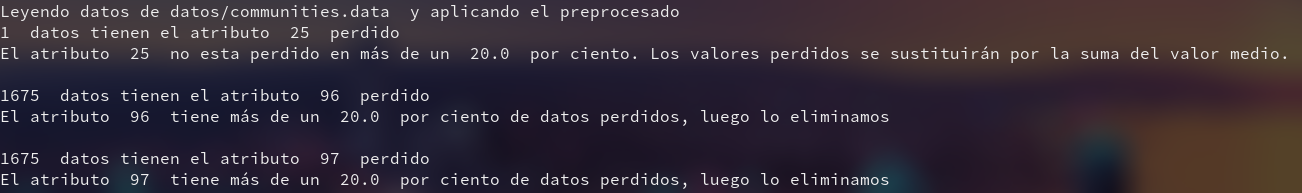
\includegraphics[scale=0.4]{regresion/preprocesado.png}
	\caption{Preprocesado de los datos en el problema de regresión.}
	\label{prepro}
\end{figure}


Observamos como el atributo 25 (atributos finales, sin contar los no predictivos) tiene un único valor perdido, luego este es sustituido por la media, mientras que otros atributos como el 96, 97 y demás que están en la salida del script pero no aquí ya que no he considerado necesario mostrarlos en la memoria, la gran cantidad de valores perdidos hace que dichos atributos sean eliminados.

Esto lo hemos podido hacer ya que al leer los datos con pandas, he sustituido los valores perdidos por nan, y para preprocesarlo simplemente he recorrido la matriz por columnas, haciendo la media de cada columna y contando el número de valores nan\cite{npIsNaN}, si el contador es más que el porcentaje dado de datos, se guarda en una lista para eliminar dichas columnas al final con la función delete de NumPy\cite{npDelete}, y en caso de ser menor, los valores nan se sustituyen por la media calculada.

Finalmente, al eliminar los atributos con muchos valores perdidos obtenemos que finalmente trabajaremos con 100 atributos.

\subsection{Fijar la métrica. Idoneidad sobre el problema.}

En este apartado fijaremos la métrica que usaremos para la evaluación, es decir, la métrica que utilizaremos para calcular el error del modelo una vez esté entrenado, es decir, saber como bien se comporta. Esto no quiere decir que la métrica que usará el modelo para entrenarse sea obligatoriamente esta, aunque en este problema si que lo será.


Debido a que estamos en un problema de regresión la métrica de evaluación será el error cuadrático medio\cite{meanSquareError}, es decir, que a mayor distancia de los datos con nuestro ajuste, mayor será el error.

He escogido esta métrica ya que es simple, como hemos visto en teoría, prácticas y la bibliografía es muy usada y como hemos comprobado en otras prácticas y veremos más adelante se comporta de forma adecuada, al estar ante un problema de regresión intentando estimar valores numéricos decimales.


\subsection{Técnica de ajuste elegida.}

Al igual que en el problema de clasificación, para realizar el ajuste usaremos la métrica Mean Squared Error, ya que los modelos lineales que he seleccionado y veremos más adelante se basan en regresión, luego no podemos usar la métrica para la evaluación escogida. 

Usaremos esta métrica de ajuste ya que es bastante conocida para nosotros y la hemos utilizado en otras prácticas de clasificación en las que hemos usado modelos lineales basados en regresión, además de comportarse bien en nuestro problema como veremos más adelante.


$$ \frac{1}{N} \sum_{i=1}^{N}{(y_i - \hat{y}_i)^2} $$

Siendo $y_i$ la clase real del dato e $\hat{y}_i$ la clase predecida por el modelo.


\subsection{Necesidad de regularización.}

La regularización es necesaria para evitar el overfitting al entrenar el modelo. La idea de utilizar regularización es minimizar el cambio en la función de error, para obligar a que no se ajuste de forma perfecta a los datos. Esta técnica nos será útil especialmente cuando los datos contienen ruido, como es nuestro caso.

Debido a la alta dimensionalidad de los datos es posible que se genere overfitting, aunque no lo sabemos a priori, por este motivo en los modelos a usar que explicaré más adelante probaré a utilizar los distintos modelos con y sin regularización.

En principio si es necesaria esta regularización, sin embargo voy a realizar distintos experimentos para comprobar su importancia.

Para aplicar la regularización existen dos normas\cite{l1l2regularizacion}.


\subsubsection{Norma L1: }

La norma L1, llamada Regresión Lasso, consiste en añadir el valor absoluto de la magnitud multiplicado por el coeficiente de penalización:

$$ \lambda \sum_{j=1}^{p}{|\beta_j|} $$

\subsubsection{Norma L2:}

La norma L2, también llamada Ridge Regression, se basa en añadir el cuadrado de la magnitud por el coeficiente de penalización en la función de coste:

$$ \lambda \sum_{j=1}^{p}{\beta_j^2} $$


En este problema utilizaremos la norma L2 ya que es la más similar a la métrica de ajuste usada. En caso de que al realizar pruebas y comprobar que la norma L1 se comporta mejor, modificaré esta sección explicando el cambio (si se llega a producir).

\newpage

\subsection{Modelos a usar.}

En esta sección comentaré los modelos lineales a usar para intentar resolver el problema.

Usaré Regresión Lineal, Regresión Ridge y Gradiente Descendente Estocástico. Usaré la implementación dada en Scikit-Learn\cite{scikitlearnlinearmodels}, y comentaré como funcionan, aunque son los algoritmos vistos en prácticas anteriores por los que ya los conocemos.

He decidido no usar el modelo Perceptron ya que, como he comentado, los datos pueden contener ruido y no ser linealmente separables, aun así podría haber usado el modelo PLA-Pocket, sin embargo considero que estudiando el comportamiento en los modelos mencionados no es necesario añadir este.


\subsubsection{Regresión Lineal.}

En este caso este modelo es el visto en otras prácticas y en teoría. Como vemos en el código del algoritmo\cite{sourceLinReg} y hemos visto en la asignatura, este algoritmo es un algoritmo simple y sencillo, por lo que no tiene muchos parámetros con los que podamos intentar ajustar mejor el modelo.


\subsubsection{Regresión Ridge.}

Este modelo es una variación de la Regresión Lineal pero teniendo en cuenta la regularización. En concreto usa la norma L2. Como podemos ver en su código fuente\cite{sourceRidgeReg}, se trata del modelo anterior teniendo en cuenta dicha norma.


\subsubsection{Gradiente Descendente Estocástico.}

De nuevo, este modelo es el visto en la asignatura, sin embargo Scikit-Learn cuenta con dos variantes, una para clasificación y otra para regresión. En este problema, al tratarse de regresión, usaremos dicha variante\cite{sourceSGDReg}.


\newpage

\subsection{Hiperparámetros y selección del mejor modelo.}

En esta sección discutiré los hiperparámetros de cada algoritmo, así como cuales considero los mejores para cada uno, y finalmente el modelo que mejor se comportan en nuestro problema.

Las ejecuciones se hacen de igual forma que en el problema anterior, luego reutilizaré la función usada:

\begin{lstlisting}
estimador = ClaseEstimador(hiperparametros)
evaluar(estimador, x, y, x_test, x_test, num_kfolds)
\end{lstlisting}


\subsubsection{Regresión Lineal}

Este modelo, como podemos ver en en la web de Scikit-Learn\cite{linearReg} es muy básico y no tenemos parámetros para realizar el ajuste, luego simplemente lo ejecutamos, obteniendo el siguiente resultado:


\begin{figure}[H]
	\centering
	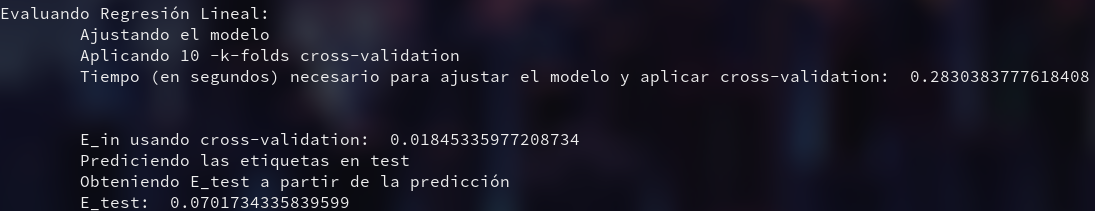
\includegraphics[scale=0.45]{regresion/regLin.png}
	\caption{Resultado usando el algoritmo Regresión Lineal.}
	\label{ridge0}
\end{figure}


Con la única ejecución de este algoritmo podemos ver como el error dentro de la muestra es muy bajo, del 1'8\%, mientras que el error en el conjunto de test es del 7'02\%. Vemos como el modelo se comporta bien fuera de la muestra incluso sin regularización, vemos si esto lo podemos mejorar aplicando dicha regularización.

\newpage

\subsubsection{Regresión Ridge.}

En este modelo, aunque ofrece gran cantidad de parámetros para controlar su funcionamiento, nos vamos a centrar en tres:

\begin{enumerate}
	\item alpha: Factor por el que se multiplica el método de regularización, en este caso la norma L2 aplicada por defecto. Este parámetro por defecto tiene valor 1.
	\item max\_iter: Máximo número de iteraciones del algoritmo. Por defecto no tiene límite de iteraciones.
	\item tol: Precisión de la solución. Por defecto $1^{-3}$.
\end{enumerate}


Podemos ver todos los parámetros disponibles en la web de Scikit-Learn\cite{ridgeReg}.


Para este modelo no modificaré la precisión de la solución ya que es bastante baja ni el máximo de iteraciones ya que no consume un tiempo considerable.

El factor que si modificaré será el factor que multiplica al método de regularización. He realizado pruebas con valores 0 (sin regularización), 0.1, 1 (valor por defecto) y 2, obteniendo estos resultados:



\begin{figure}[H]
	\centering
	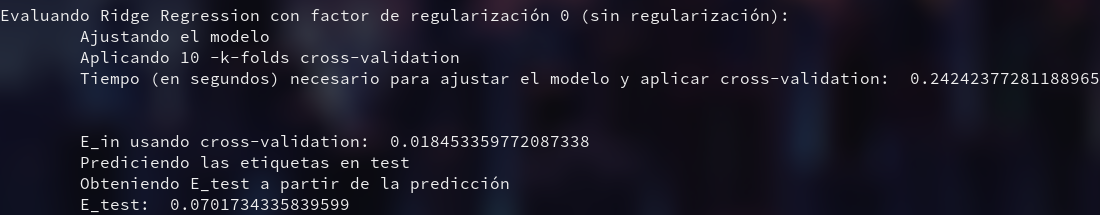
\includegraphics[scale=0.45]{regresion/ridge0.png}
	\caption{Resultado usando el algoritmo Ridge Regression sin regularización.}
	\label{ridge0}
\end{figure}


\begin{figure}[H]
	\centering
	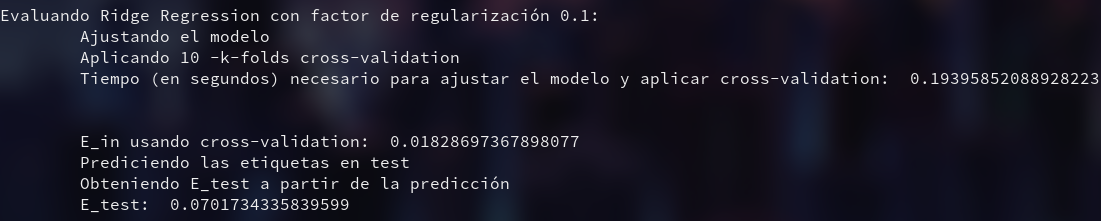
\includegraphics[scale=0.45]{regresion/ridge01.png}
	\caption{Resultado usando el algoritmo Ridge Regression con factor de regularización 0.1.}
	\label{ridgereg01}
\end{figure}



\begin{figure}[H]
	\centering
	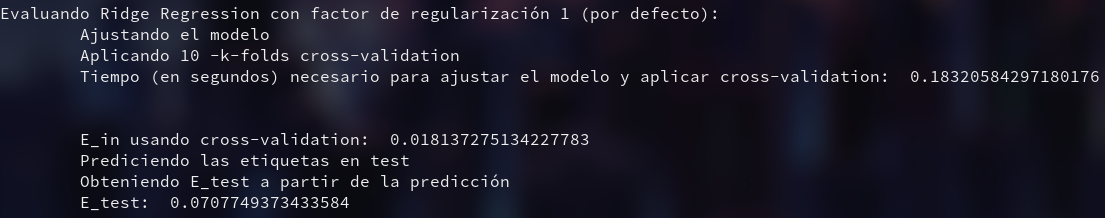
\includegraphics[scale=0.45]{regresion/ridge1.png}
	\caption{Resultado usando el algoritmo Ridge Regression con factor de regularización 1.}
	\label{ridgereg1}
\end{figure}



\begin{figure}[H]
	\centering
	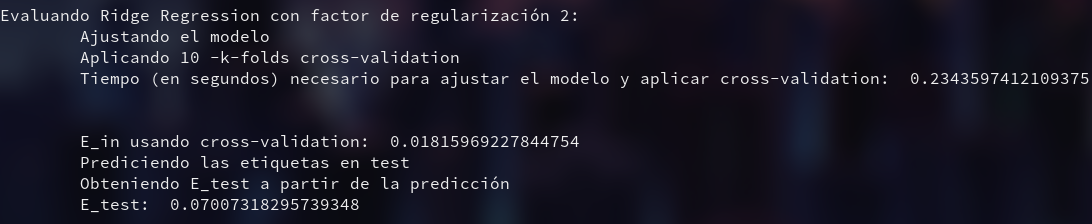
\includegraphics[scale=0.45]{regresion/ridge2.png}
	\caption{Resultado usando el algoritmo Ridge Regression con factor de regularización 2.}
	\label{ridgereg2}
\end{figure}


En principio, viendo los resultados, vemos como este algoritmo se comporta bien, aunque con el mismo problema que Regresión Lineal, tiene una tasa de error muy baja dentro de la muestra pero bastante mayor en el conjunto de test, aún aplicando la regularización.

Debido a que al aplicar una mayor regularización (usando un factor 2) obtenemos mejores resultados en test, he añadido el siguiente experimento con factor 3:


\begin{figure}[H]
	\centering
	\includegraphics[scale=0.45]{regresion/ridge3.png}
	\caption{Resultado usando el algoritmo Ridge Regression con factor de regularización 3.}
	\label{ridgereg3}
\end{figure}


Vemos como volvemos a tener peor resultado en el error en test, 

\newpage

\subsubsection{Gradiente Descendente Estocástico.}

En Gradiente Descendente Estocástico tenemos los siguientes parámetros cruciales:

\begin{enumerate}
	\item loss: Función de perdida. Por defecto 'hinge'.
	\item penalty: Termino de regularización. Por defecto la norma L2.
	\item alpha: Constante multiplicadora de la regularización. Por defecto 0.0001. Con un mayor valor, mayor será la regularización.
	\item learning\_rate: Esquema para la tasa aprendizaje. Por defecto optimo, siguiendo la siguiente formula $eta = \frac{1}{alpha \cdot (t + t_0)}$ donde $t_0$ es una heurística propuesta por Leon Bottou. Como podemos ver, si el esquema es el esquema óptimo el parámetro alpha debe ser distinto a 0.
	\item eta0: Valor de la tasa de aprendizaje en caso de utilizar un esquema constante. No es usado en el esquema óptimo.
	\item max\_iter: Máximo de iteraciones del algoritmo.
\end{enumerate}

Podemos ver todos los parámetros disponibles en la web de Scikit-Learn\cite{sgdclasificacion}.

Para la función de perdida usaremos square\_loss, sin embargo, como comentamos y veremos ahora, esta función de perdida se comporta muy mal, luego también ejecutaremos el algoritmo con la función de perdida Hinge.

Para el termino de regularización, como hemos hecho con todos los modelos, usaremos la norma L2.

El parámetro alpha discutiremos más adelante cual será el mejor valor, y realizaré pruebas con valores 0, 0.0001, 0.01, 0.1 y 1.

Para el esquema de la tasa de aprendizaje realizaremos las pruebas con dos esquemas, el constante y el óptimo. Las pruebas con alpha con valor 0 solo las haré con el esquema constante ya que con el óptimo es necesario para calcular el valor de la tasa de aprendizaje.

Como nota añadir que haciendo el experimento con la función de perdida square\_loss obtenemos malos resultados siempre y voy a desechar ese modelo por sus malos resultados, así que la comparación entre el esquema constante y el óptimo será con la función de perdida Hinge.


\begin{figure}[H]
	\centering
	\hspace*{-1cm}\includegraphics[scale=0.4]{regresion/sgdLoss0001.png}
	\caption{Resultado usando el algoritmo SGD con factor de regularización 0.001 y función de perdida square loss.}
	\label{SGDL0001}
\end{figure}

\begin{figure}[H]
	\centering
	\hspace*{-1cm}\includegraphics[scale=0.4]{regresion/sgdLoss001.png}
	\caption{Resultado usando el algoritmo SGD con factor de regularización 0.01 y función de perdida square loss.}
	\label{SGDL001}
\end{figure}


\begin{figure}[H]
	\centering
	\hspace*{-1cm}\includegraphics[scale=0.4]{regresion/sgdLoss01.png}
	\caption{Resultado usando el algoritmo SGD con factor de regularización 0.1 y función de perdida square loss.}
	\label{SGDL01}
\end{figure}


\begin{figure}[H]
	\centering
	\hspace*{-1cm}\includegraphics[scale=0.4]{regresion/sgdLoss1.png}
	\caption{Resultado usando el algoritmo SGD con factor de regularización 1 y función de perdida square loss.}
	\label{SGDL1}
\end{figure}

\newpage

Vemos como este modelo, aun variando el factor de regularización, obtenemos ajustes muy malos. A continuación probamos con la función de perdida Hinge:

\begin{figure}[H]
	\centering
	\hspace*{-1cm}\includegraphics[scale=0.4]{regresion/sgdH001a0.png}
	\caption{Resultado usando el algoritmo SGD Classifier con tasa de aprendizaje constante 0.01, sin regularización y función de perdida Hinge.}
	\label{SGDL0}
\end{figure}

\begin{figure}[H]
	\centering
	\hspace*{-1cm}\includegraphics[scale=0.4]{regresion/sgdH00001.png}
	\caption{Resultado usando el algoritmo SGD Classifier con tasa de aprendizaje optima (variable) y factor de regularización 0.0001 y función de perdida Hinge.}
	\label{SGDL00001}
\end{figure}

\begin{figure}[H]
	\centering
	\hspace*{-1cm}\includegraphics[scale=0.4]{regresion/sgdH00001c.png}
	\caption{Resultado usando el algoritmo SGD Classifier con tasa de aprendizaje constante y factor de regularización 0.0001 y función de perdida Hinge.}
	\label{SGDL00001}
\end{figure}

\begin{figure}[H]
	\centering
	\hspace*{-1cm}\includegraphics[scale=0.4]{regresion/sgdH001.png}
	\caption{Resultado usando el algoritmo SGD Classifier con tasa de aprendizaje optima (variable) y factor de regularización 0.01 y función de perdida Hinge.}
	\label{SGDL001}
\end{figure}

\begin{figure}[H]
	\centering
	\hspace*{-1cm}\includegraphics[scale=0.4]{regresion/sgdH001c.png}
	\caption{Resultado usando el algoritmo SGD Classifier con tasa de aprendizaje constante y factor de regularización 0.01 y función de perdida Hinge.}
	\label{SGDL001}
\end{figure}


\begin{figure}[H]
	\centering
	\hspace*{-1cm}\includegraphics[scale=0.4]{regresion/sgdH01.png}
	\caption{Resultado usando el algoritmo SGD Classifier con tasa de aprendizaje optima (variable) y factor de regularización 0.1 y función de perdida Hinge.}
	\label{SGDL001}
\end{figure}

\begin{figure}[H]
	\centering
	\hspace*{-1cm}\includegraphics[scale=0.4]{regresion/sgdH01c.png}
	\caption{Resultado usando el algoritmo SGD Classifier con tasa de aprendizaje constante y factor de regularización 0.1 y función de perdida Hinge.}
	\label{SGDL001}
\end{figure}


\begin{figure}[H]
	\centering
	\hspace*{-1cm}\includegraphics[scale=0.4]{regresion/sgdH1.png}
	\caption{Resultado usando el algoritmo SGD Classifier con tasa de aprendizaje optima (variable) y factor de regularización 1 y función de perdida Hinge.}
	\label{SGDL001}
\end{figure}

\begin{figure}[H]
	\centering
	\hspace*{-1cm}\includegraphics[scale=0.4]{regresion/sgdH1c.png}
	\caption{Resultado usando el algoritmo SGD Classifier con tasa de aprendizaje constante y factor de regularización 1 y función de perdida Hinge.}
	\label{SGDL001}
\end{figure}


Vemos como en todos los casos con un esquema de tasa de aprendizaje óptimo obtenemos muy buenos resultados que se parecen mucho, los cuales ahora comentaremos.

Con el esquema constante, vemos como el factor de regularización si influye en gran medida, ya que como vemos, con un factor 1 existe demasiada regularización y por lo tanto no llega a ajustar de forma correcta el modelo, dando un error tanto en la muestra como en test bastante alto (del 40\% y 55\% respectivamente), mientras que sin regularizar obtenemos un 8'6\% de error en test, y con la regularización por defecto obtenemos un mejor valor, 5'2\% de error en test, aunque en el primero obtengamos mejor valor del error dentro de la muestra, por lo que podemos ver que la regularización sigue siendo necesaria y evita overfitting en el entrenamiento.


\subsubsection{Mejor modelo.}

Escogeré el mejor modelo según el modelo con mejor error en el conjunto de test ya que es el que mejor ha estimado unos datos con los que no ha entrenado. Por este motivo el modelo escogido será Regresión Logística con un factor de regularización $C=1$, por lo que la estimación del error se hará con este modelo.

\newpage

\subsection{Estimación del error fuera de la muestra usando validación cruzada y comparación con el error en test.}

Como hemos visto tanto en teoría\cite{teoria} como en la bibliografía de la asignatura\cite{libro}, podemos hacer una estimación del error fuera de la muestra al usar validación cruzada.

Si tenemos $N$ conjuntos de validación, sabemos que:

$$E_{cv} = \frac{1}{N}\sum_{n=1}^{N}{E_{val}(g_n^-)}$$

Y como hemos visto acorde a las curvas de aprendizaje vistas en teoría, sabemos que:

$$E_{out}(g) \leq E_{cv}(g) $$

En realidad $E_{cv}$ es la media de todos los errores al usar la función \texttt{cross\_val\_score}, luego esta estimación se ha hecho para todas las pruebas que hemos realizado y en concreto en el modelo escogido obtenemos que:

$$  E_{out}(g) \leq 0'038$$

Vemos como claramente esto no es así, ya que en el mismo modelo el error en el conjunto de test es mayor (0'0512), y esto puede deberse a que el número de $k$-folds es demasiado alto.




\subsection{Modelo propuesto y estimación del error fuera de la muestra de este modelo.}

Podemos hacer una estimación del error fuera de la muestra usando el conjunto de test. En el modelo que hemos escogido vemos como esta estimación se de un error del 5'12\%.

Esto lo podemos comprobar mostrando la matriz de confusión.

Esta matriz hará un recuento de los datos reales y predecidos. En las filas se muestra el valor real de la clase, y el las columnas el valor predecido por nuestro modelo, de forma que si el valor real es un 0 y el modelo ha predecido un 7, sumará uno en la posición 0,7. 

\begin{figure}[H]
	\centering
	\includegraphics[scale=0.45]{regresion/matrizC.png}
	\caption{Matriz de confusión con los datos predecidos del modelo seleccionado.}
	\label{MC}
\end{figure}

El que en esta matriz se muestre la diagonal con los números mayores quiere decir que la mayor parte del conjunto de test ha realizado una buena predicción, mientras que en las posiciones  fuera de la diagonal ha cometido error. Vemos como principalmente comete errores al clasificar el número 8, que lo suele confundir con un 1 (imagino que al ser ambos bastante similares, ser simétricos y estar por la zona central de la imagen) y con un 9 (al compartir la misma zona de la imagen y solo diferenciarse en un cuadrante de la imagen).

Aun así, hemos obtenido muy buenos resultados para ser un problema con gran número de variables y tener gran cantidad de clases.

\newpage


\section{Referencias, material y documentación usada}


\begin{thebibliography}{9}


\bibitem{teoria}
Diapositivas de teoría

\bibitem{libro}
Learning From Data by Yaser S. Abu-Mostafa, Malik Magdon-Ismail, Hsuan-Tien Lin

\bibitem{sklearn}
Página web de Scikit Learn

\url{https://scikit-learn.org/stable/user_guide.html}


\bibitem{sklearn-linearmodel}
Scikit-Learn: Modelos lineales
\url{https://scikit-learn.org/stable/modules/linear_model.html}


\bibitem{pandasReadCSV}
Pandas: read\_csv

\url{https://pandas.pydata.org/pandas-docs/stable/reference/api/pandas.read_csv.html}

\bibitem{mlr_digitos}
Machine Learning Repository: Optical Recognition of Handwritten Digits Data Set 

\url{https://archive.ics.uci.edu/ml/datasets/optical+recognition+of+handwritten+digits}


\bibitem{crossval}
Scikit-Learn: Cross-validation:

\url{https://scikit-learn.org/stable/modules/generated/sklearn.model_selection.cross_val_score.html}



\bibitem{ridge}
Scikit-Learn: Clasificador Ridge

\url{https://scikit-learn.org/stable/modules/generated/sklearn.linear_model.RidgeClassifier.html#sklearn.linear_model.RidgeClassifier}

\bibitem{logisticregression}
Scikit-Learn: Regresión Logística

\url{https://scikit-learn.org/stable/modules/generated/sklearn.linear_model.LogisticRegression.html#sklearn.linear_model.LogisticRegression}

\bibitem{sgdclasificacion}
Scikit-Learn: Clasificador SGD 

\url{https://scikit-learn.org/stable/modules/generated/sklearn.linear_model.SGDClassifier.html#sklearn.linear_model.SGDClassifier}


\bibitem{l1l2regularizacion}
Métodos de regularización: Norma L1 y L2:

\url{https://towardsdatascience.com/l1-and-l2-regularization-methods-ce25e7fc831c}


\bibitem{scikitlearnlinearmodels}
Scikit-Learn: Linear Models

\url{https://scikit-learn.org/stable/modules/linear_model.html}


\bibitem{sourceRidge}
Código fuente Ridge Classification Scikit-Learn:

\url{https://github.com/scikit-learn/scikit-learn/blob/fd237278e/sklearn/linear_model/_ridge.py#L765}



\bibitem{sourceLogistic}
Código fuente Logistic Regression Scikit-Learn:

\url{https://github.com/scikit-learn/scikit-learn/blob/fd237278e/sklearn/linear_model/_logistic.py#L1011}



\bibitem{sourceSGDClas}
Código fuente SGD para clasificación Scikit-Learn:

\url{https://github.com/scikit-learn/scikit-learn/blob/fd237278e/sklearn/linear_model/_stochastic_gradient.py#L731}



\bibitem{scoring-cross-val}
Scikit-Learn: Métricas para la validación cruzada

\url{https://scikit-learn.org/stable/modules/model_evaluation.html#scoring-parameter}


\bibitem{hingeLoss}
Función de perdida Hinge:

\url{https://en.wikipedia.org/wiki/Hinge_loss}


\bibitem{mlr_crimen}
Machine Learning Repository: Communities and Crime Data Set  

\url{http://archive.ics.uci.edu/ml/datasets/Communities+and+Crime}


\bibitem{linearReg}
Scikit-Learn: Regresión Lineal

\url{https://scikit-learn.org/stable/modules/generated/sklearn.linear_model.LinearRegression.html#sklearn.linear_model.LinearRegression}

\bibitem{ridgeReg}
Scikit-Learn: Ridge Regression

\url{https://scikit-learn.org/stable/modules/generated/sklearn.linear_model.Ridge.html#sklearn.linear_model.Ridge}

\bibitem{sgdregresion}
Scikit-Learn: SGD Regression

\url{https://scikit-learn.org/stable/modules/generated/sklearn.linear_model.SGDRegressor.html#sklearn.linear_model.SGDRegressor}


\bibitem{sourceLinReg}
Código fuente Lineal Regression Scikit-Learn:

\url{https://github.com/scikit-learn/scikit-learn/blob/fd237278e/sklearn/linear_model/_base.py#L389}

\bibitem{sourceRidgeReg}
Código fuente Ridge Regressor Scikit-Learn:

\url{https://github.com/scikit-learn/scikit-learn/blob/fd237278e/sklearn/linear_model/_ridge.py#L603}



\bibitem{sourceSGDReg}
Código fuente SGD para regresión Scikit-Learn:

\url{https://github.com/scikit-learn/scikit-learn/blob/fd237278e/sklearn/linear_model/_stochastic_gradient.py#L1354}



\bibitem{trainTestSplit}
Scikit-Learn: Separar conjunto en entrenamiento y test

\url{https://scikit-learn.org/stable/modules/generated/sklearn.model_selection.train_test_split.html?highlight=train_test_split#sklearn.model_selection.train_test_split}


\bibitem{npIsNaN}
NumPy: isnan

\url{https://numpy.org/doc/stable/reference/generated/numpy.isnan.html}

\bibitem{npDelete}
NumPy: delete

\url{https://numpy.org/doc/stable/reference/generated/numpy.delete.html}


\bibitem{meanSquareError}
Scikit-Learn: Métrica error cuadrático medio.

\url{https://scikit-learn.org/stable/modules/generated/sklearn.metrics.mean_squared_error.html#sklearn.metrics.mean_squared_error}

\end{thebibliography}

\end{document}
